\documentclass[10pt]{beamer}

\usetheme[progressbar=foot]{metropolis}

\usepackage{amsmath,amsfonts,amssymb,pxfonts,eulervm,xspace}
\usepackage{graphicx}
\usepackage{tikz}
% \usepackage{adjustbox}      
\usepackage{filecontents}
\usepackage{fancyhdr}
\usepackage{xcolor}
\usepackage{makecell}
\usepackage{tabularx}
\usepackage{listings}

\graphicspath{{figures/}}

\lstset{
				%framexleftmargin=10mm,
				breaklines=true,
				language=C++, 
				alsoletter=0123456789,
			    otherkeywords={1, 2, 3, 4, 5, 6, 7, 8, 9, 0},
				%frame=tb, % draw a frame at the top and bottom of the code block
   				tabsize=2, % tab space width
			    showstringspaces=false, % don't mark spaces in strings
    			numbers=left, % display line numbers on the left    			
    			numberstyle=\color{black},
                keywordstyle=\color{blue},
                stringstyle=\color{yellow!60!red},
                commentstyle=\color{gray},
                basicstyle=\color{red},
                identifierstyle=\color{black},
                morecomment=[l][\color{green!40!black}]{\#},
			    keepspaces=true,
			    numbersep=2ex,
			    xleftmargin=2.5ex,
				framexleftmargin=5ex,  
				%xleftmargin=\parindent,
   				showtabs=true,
   				literate=%
    *{0}{{{\digitcolor{0}}}}1
    {1}{{{\digitcolor{1}}}}1
    {2}{{{\digitcolor{2}}}}1
    {3}{{{\digitcolor{3}}}}1
    {4}{{{\digitcolor{4}}}}1
    {5}{{{\digitcolor{5}}}}1
    {6}{{{\digitcolor{6}}}}1
    {7}{{{\digitcolor{7}}}}1
    {8}{{{\digitcolor{8}}}}1
    {9}{{{\digitcolor{9}}}}1
}

%-- Header and footer information ----------------------------------
% \newcommand{\footleft}{http://www.shawnlankton.com/category/latex/}
% \newcommand{\footcenter}{http://www.shawnlankton.com/category/latex/}
% \newcommand{\footright}{alexandru.p.ionita@gmail.com}

\usepackage{appendixnumberbeamer}
\usepackage{booktabs}
\usepackage[scale=2]{ccicons}
\usepackage{amsmath,amsfonts,amssymb,pxfonts,eulervm,xspace}
\usepackage{graphicx}
\usepackage{tikz}
\usepackage{adjustbox}      
\usepackage{filecontents}
% \usepackage{listings}
\usepackage{fancyhdr}
\usepackage{xcolor}

\usepackage{infogym}

\title{Course Name}
\author{Nume \quad Prenume }
% \author{Nume \quad Prenume - }
\institute{Centrul Infogym Iasi}



% \AtBeginSection[]
% {
%   \begin{frame}
% 	\begin{columns}
% 	\begin{column}{0.40\linewidth}
%   \begin{block}{Content}
% 	\tableofcontents[subsectionstyle=show/shaded, sectionstyle=show/shaded]
% 	\end{block}
% 	\end{column}
% 	\begin{column}{0.40\linewidth}
% 	\end{column}
% 	\end{columns}
%   \end{frame}
% }


%-- Main Document --------------------------------------------------
\begin{document}


\begin{frame}
    \titlepage
\end{frame}


\begin{frame}
\begin{center}
 Computer Science - Algorithms\\
 11-12 Classes\\
 Advanced Course
\\
\color{gray}
Subtitle \\
 Course description 1\\
Course description 2\\

\end{center}
\end{frame}


%\section{Overview}

\begin{frame}[allowframebreaks]
Content
    \tableofcontents
  % You might wish to add the option [pausesections]
\end{frame}



\section{Introdution}

\subsection{What is this about?}

\begin{frame}{\insertsubsection}

      \begin{block}{block title}
      	Description

      	another description 

      	$\forall\ key \in T_{left} \leq T_{key} < \forall\ T_{key} \in T_{right}$     

      	$ T_{pri} > \forall\ T_{pri} \in (T_{right} \cup T_{left})$      	
      	
      \end{block}

\end{frame}



\subsection{Problems solved using treaps}
\begin{frame}
	
	\begin{block}{Problems solved using treaps}
		\begin{itemize}
			\item arrays with indexes in range [$0, 10^{18}$]. $O(N)$ space
			\item keeps sorted array. $O(N)$ space, $O(logN)$ time for insert \& delete
			\item Sum, Min, Max on interval. $O(logN)$ time
			\item Number of elements smaller than $X$. $O(logN)$ time
			\item Reverse elements on interval. $O(logN)$ time.
			\item Find $K$th element. $O(logN)$ time
			\item Insert an element at $K$th position in an array. $O(logN)$ time
			\item playing around with split \& merge.
		\end{itemize}
		
		where $N$ - numbber of elements.
		
	\end{block}
\end{frame}



\subsection{Basic operations}
\begin{frame}
	Basic Operations	

		\begin{tabular}{@{} R{.2\linewidth} L{.7\linewidth}  @{}}
	  $\mathbf{Split(T,X)}$ $\mathcal{O}(\log N)$ &  Splits a treap \textbf{T} int two treaps, $\mathbf{T_1}$ and $\mathbf{T_2}$ 
	  by a key value $\mathbf{X}$, such as $\forall\ element \in T_1 \leq X < \forall\ element \in T_2$.\\
	 
	  $\mathbf{Merge(T_1,T_2)}$ $\mathcal{O}(\log N)$ & 
	 Merges two treaps, $\mathbf{T_1}$ and $\mathbf{T_2}$ which respect the condition: $\forall\ element \in T_1 \leq X < \forall\ element \in T_2$, into a treap $\mathbf{T}$\\

	  $\mathbf{Search(T,X)}$   $\mathcal{O}(\log N)$ &
	   Searches in $\mathbf{T}$ a node with the key value $\mathbf{X}$. The implementation is the same as for an ordinary binary tree. \\

	  $\mathbf{Insert(T,X)}$ $\mathcal{O}(\log N)$ &
	   Inserts in $\mathbf{T}$ a new node with the key value $\mathbf{X}$. \\

	  $\mathbf{Erase(T,X)}$ $\mathcal{O}(\log N)$ &
	   Searches in $\mathbf{T}$ a node with the key value $\mathbf{X}$ and removes it from the tree.
		\end{tabular}
	
\end{frame}

\subsection{Advanced operations}
\begin{frame}

	Advanced Operations	

		\begin{tabular}{@{} R{.2\linewidth} L{.7\linewidth}  @{}}

	$\mathbf{Build (X_1, ..., X_N)}$ $\mathcal{O}(N)$ &
	   Builds a tree from a list of sorted values. This can be done in linear time (assuming that $X_1,...,X_N$ are sorted).\\
	  $\mathbf{Union (T_1, T_2)}$ in $\mathcal{O}(M*log(N/M))$ &
 Merges two trees, assuming that all the elements are different. 
 An implementation with the same asymptotic behavior is possible if duplicate elements should be removed during merge.\\
	  $\mathbf{Intersect (T_1, T_2)}$ in $\mathcal{O}(M*log(N/M))$ &
 Finds the intersection of two trees (i.e. their common elements). We will not consider the implementation of this operation here.
		\end{tabular}

		
	\end{frame}



\section{Extensions}


\begin{frame}
\begin{block}{Implicit Key Treap}
A simple and very powerful modification. The idea is that the keys should be indices of the elements in the array. The keys are not kept explicit in the structure, they are calculated using the variable which keeps the size of the subtree.\\
In addition to the normal treap: 
		\begin{itemize}
			\item Find $K$th element. $O(logN)$ time
			\item Insert an element at $K$th position in an array. $O(logN)$ time
		\end{itemize}
\end{block}
\begin{block}{Lazy Update Treap}
	Exacty the same as lazy update on a Binary Indexed Tree.
	Supports:
		\begin{itemize}
			\item Update on interval. $O(logN)$ time
			\item Reverse elements on interval. $O(logN)$ time.
		\end{itemize}
\end{block}
\end{frame}



\begin{frame}[fragile]
\begin{columns}
	\begin{column}{0.60\linewidth}	
		\begin{block}{Split - Normal Treap}
			\begin{lstlisting}[language=c++]
void split(treap * root, int key, 
           treap * &left, treap* &right)
{
  if(root == null)
    left = right = null;
  else if(key <= root->key) //split left child
  	split(root->left, key, left, root->left),
  	right = root;
  else                      //split right child
    split(root->right, key, root->right, right),
    left = root;
  update(root);
}
			\end{lstlisting}
		\end{block}
	\end{column}	
	\begin{column}{0.38\linewidth}	
	\begin{figure}[htb]
          \centering
          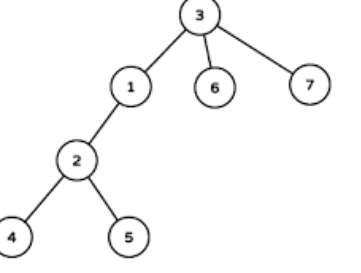
\includegraphics[width=1\linewidth]{images/graph.png}
        \end{figure}
	\end{column}	
	\end{columns}	
\end{frame}


\section{Case Study}


\begin{frame}{Codeforces 702F - T-shirts}

\begin{itemize}
	\item Problema cu siruri pare/impare
	\item \url{https://acm.timus.ru/problem.aspx?space=1&num=1439}
	\item Codeforces 702F \url{http://codeforces.com/contest/702/problem/F}	
\end{itemize}



\end{frame}



\section{Practice Problems}


%%% >>>>> Practice Problems ---------------------------
\begin{frame}[allowframebreaks]

\begin{thebibliography}{9}

\bibitem{knuthwebsite} 
TREAP SPOJ\url{http://www.spoj.com/problems/TREAP/}
\bibitem{knuthwebsite} 
Zeap - infoarena, \url{http://www.infoarena.ro/problema/zeap}
\bibitem{knuthwebsite} 
Codeforces 101174F, \url{http://codeforces.com/problemset/gymProblem/101174/F}
\bibitem{knuthwebsite} 
Timus 1645, \url{http://acm.timus.ru/problem.aspx?space=1&num=1645}
\bibitem{knuthwebsite} 
Timus 1439 \url{http://acm.timus.ru/problem.aspx?space=1&num=1439}
\bibitem{knuthwebsite} 
Codeforces 702F \url{http://codeforces.com/contest/702/problem/F}
\bibitem{knuthwebsite} 
Codeforces 455D \url{http://codeforces.com/contest/455/problem/D}
\bibitem{knuthwebsite} 
Timus 1521 \url{http://acm.timus.ru/problem.aspx?space=1&num=1521}
\bibitem{knuthwebsite} 
Monster Mindcoding Final Round 2017 \url{https://mindcoding.ro/pb/monster}


\url{https://acm.timus.ru/problem.aspx?space=1&num=1439} %clasic treap implicit

\end{thebibliography}

\begin{block}{Bibliography}
\begin{thebibliography}{9}

\bibitem{knuthwebsite} 
\url{https://e-maxx-eng.appspot.com/data_structures/treap.html}
\bibitem{knuthwebsite} 
\url{http://codeforces.com/blog/entry/11148}
\bibitem{knuthwebsite} 
\url{http://codeforces.com/blog/entry/3767}


\end{thebibliography}
\end{block}
\end{frame}


%%% <<<<< Practice Problems ---------------------------




\end{document}
